\documentclass{article}
\usepackage[margin=1.0in]{geometry}
\usepackage{amsmath, amssymb, mathrsfs}
\usepackage[english]{babel}
\usepackage{graphicx}
\usepackage{enumerate}
\usepackage{listings}
\usepackage{tikz}
\renewcommand{\vec}[1]{\mathbf{#1}}
\newcommand{\floor}[1]{\left\lfloor #1 \right\rfloor}
\newcommand{\ceil}[1]{\left\lceil #1 \right\rceil}

\title{Machine Learning from Data Assignment 10}
\author{Greg Stewart}
\date{\today}

\begin{document}

\maketitle

\subsection*{Exercise 6.1}

\begin{enumerate}[(a)]
  \item \textit{Give two vectors with high cosine similarity but low Euclidean distance 
    similarity. Similarly, do the opposite.}

    \textbf{High cosine similarity; low distance similarity.}

    \[\vec{x}_1 = 
      \begin{pmatrix} 0 \\ 1 \end{pmatrix}
      \qquad
      \vec{x}_2 = 
      \begin{pmatrix} 100.01 \\ 101.01 \end{pmatrix}
    \]

    \textbf{Low cosine similarity; high distance similarity}

    \[\vec{x}_1 =
      \begin{pmatrix} 0 \\ 1 \end{pmatrix}
      \qquad 
      \vec{x}_2 =
      \begin{pmatrix} 1 \\ 0 \end{pmatrix}
    \]

  \item \textit{If origin of coordinate system changes, which measure of similarity changes? 
    How does this affect your choice of features?}

    Euclidean distance is relative, so this measure of similarity \textbf{does not} change.

    Cosine similarity, however, does change, because the angles of the vectors will change
    relative to the origin. What this change does depends on where the origin goes.

\end{enumerate}

\subsection*{Exercise 6.2}

\smallskip

\textit{Let
\[
  f(\vec{x}) = 
  \begin{cases}
    +1 & \text{if } \pi(\vec{x}) \geq \frac{1}{2} \\
    -1 & \text{otherwise} \\
  \end{cases}
\]
Show that the probability of error on a test point $\vec{x}$ is 
\[
  e(f(\vec{x})) = \mathbb{P}[f(\vec{x}) \neq y] = \min\{\pi(\vec{x}), 1-\pi(\vec{x})\}
\]
and $e(f(\vec{x}) \leq e(h(\vec{x}))$ for any other hypothesis $h$.}

\bigskip

Take $\pi(\vec{x}) \geq 1/2$, giving $f(\vec{x}) = +1$. For $y$ we have either +1 or -1, so we
need the probability that $y = -1$, in this case, so the results don't match up. Given the 
definition of $\pi(\vec{x})$, for this case we have $\mathbb{P}[f(\vec{x}) \neq y] = 1 - 
\pi(\vec{x})$.

Now consider $\pi(\vec{x}) < 1/2$, so $f(\vec{x}) = -1$. Now we need the probability that $y=+1$,
as this value means $f(\vec{x}) \neq y$. This is given by $\mathbb{P}[f(\vec{x}) \neq y] = 
\pi(\vec{x})$.

Thus, for any test point $\vec{x}$ we get the error
\[
  e(f(\vec{x})) = \mathbb{P}[f(\vec{x}) \neq y] = \min\{\pi(\vec{x}), 1-\pi(\vec{x})\}
\]

Now, $f(\vec{x})$ is the optimal prediction for the value of $y$ as it is directly tied to 
$\pi(\vec{x})$. If any nondeterministic hypothesis $h$ is chosen, then it can only be as good
as $f(\vec{x})$, or worse. Deterministic hypotheses can likewise only be as good as $f(\vec{x})$ 
in the best case. Thus
\[
  e(h(\vec{x})) = \mathbb{P}[h(\vec{x}) \neq y] \geq \min\{\pi(\vec{x}), 1-\pi(\vec{x})\}
\]

This implies that 
\[
  e(f(\vec{x})) \leq e(h(\vec{x}))
\]

\subsection*{Problem 6.1}

\smallskip

Consider the data set of 7 points given in the text.

\begin{enumerate}[(a)]
  \item \textit{Show the decision regions for the 1-NN and 3-NN rules.}

    \begin{center}
    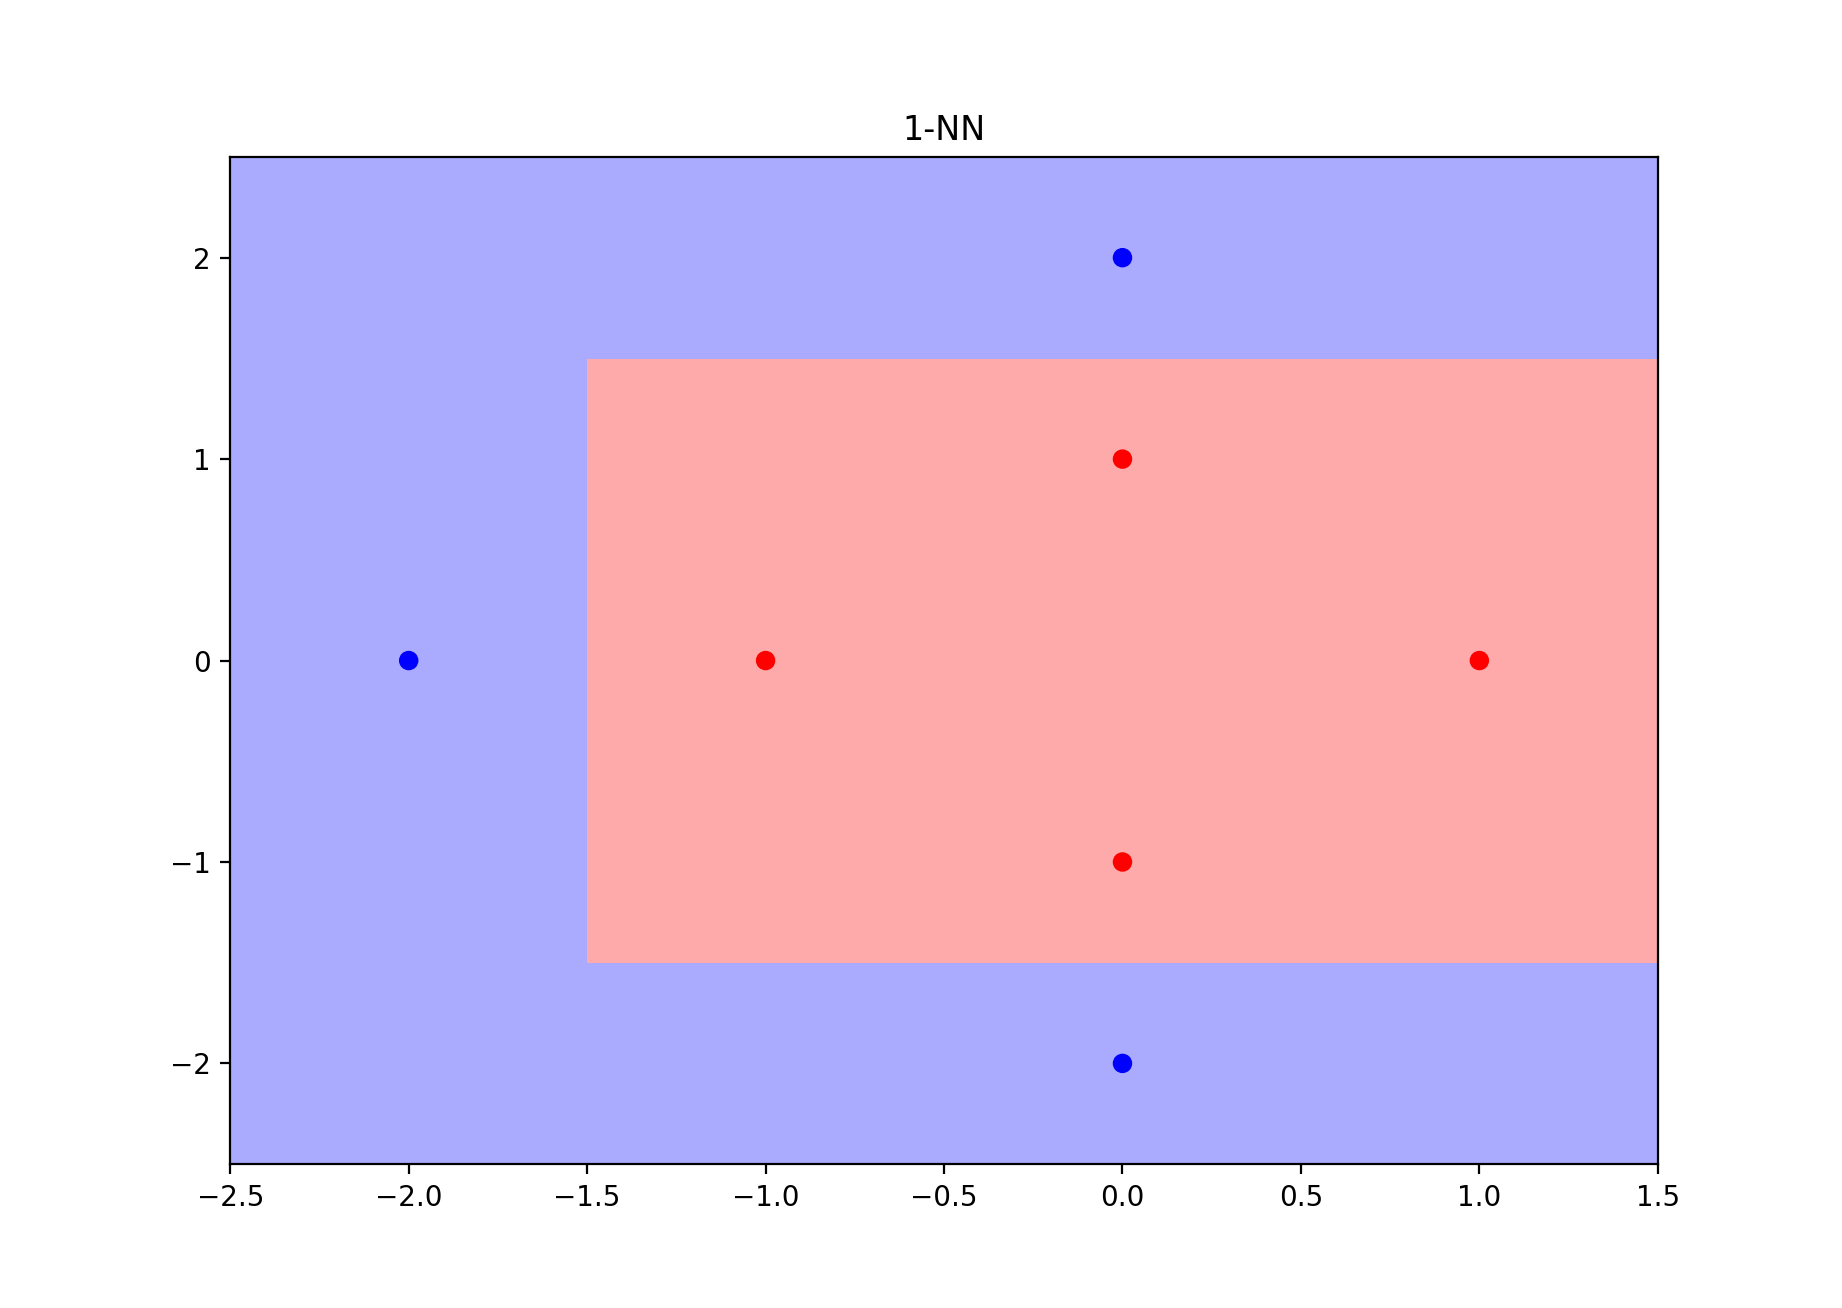
\includegraphics[width=\textwidth]{61a1nn.png}
    \end{center}

    \begin{center}
    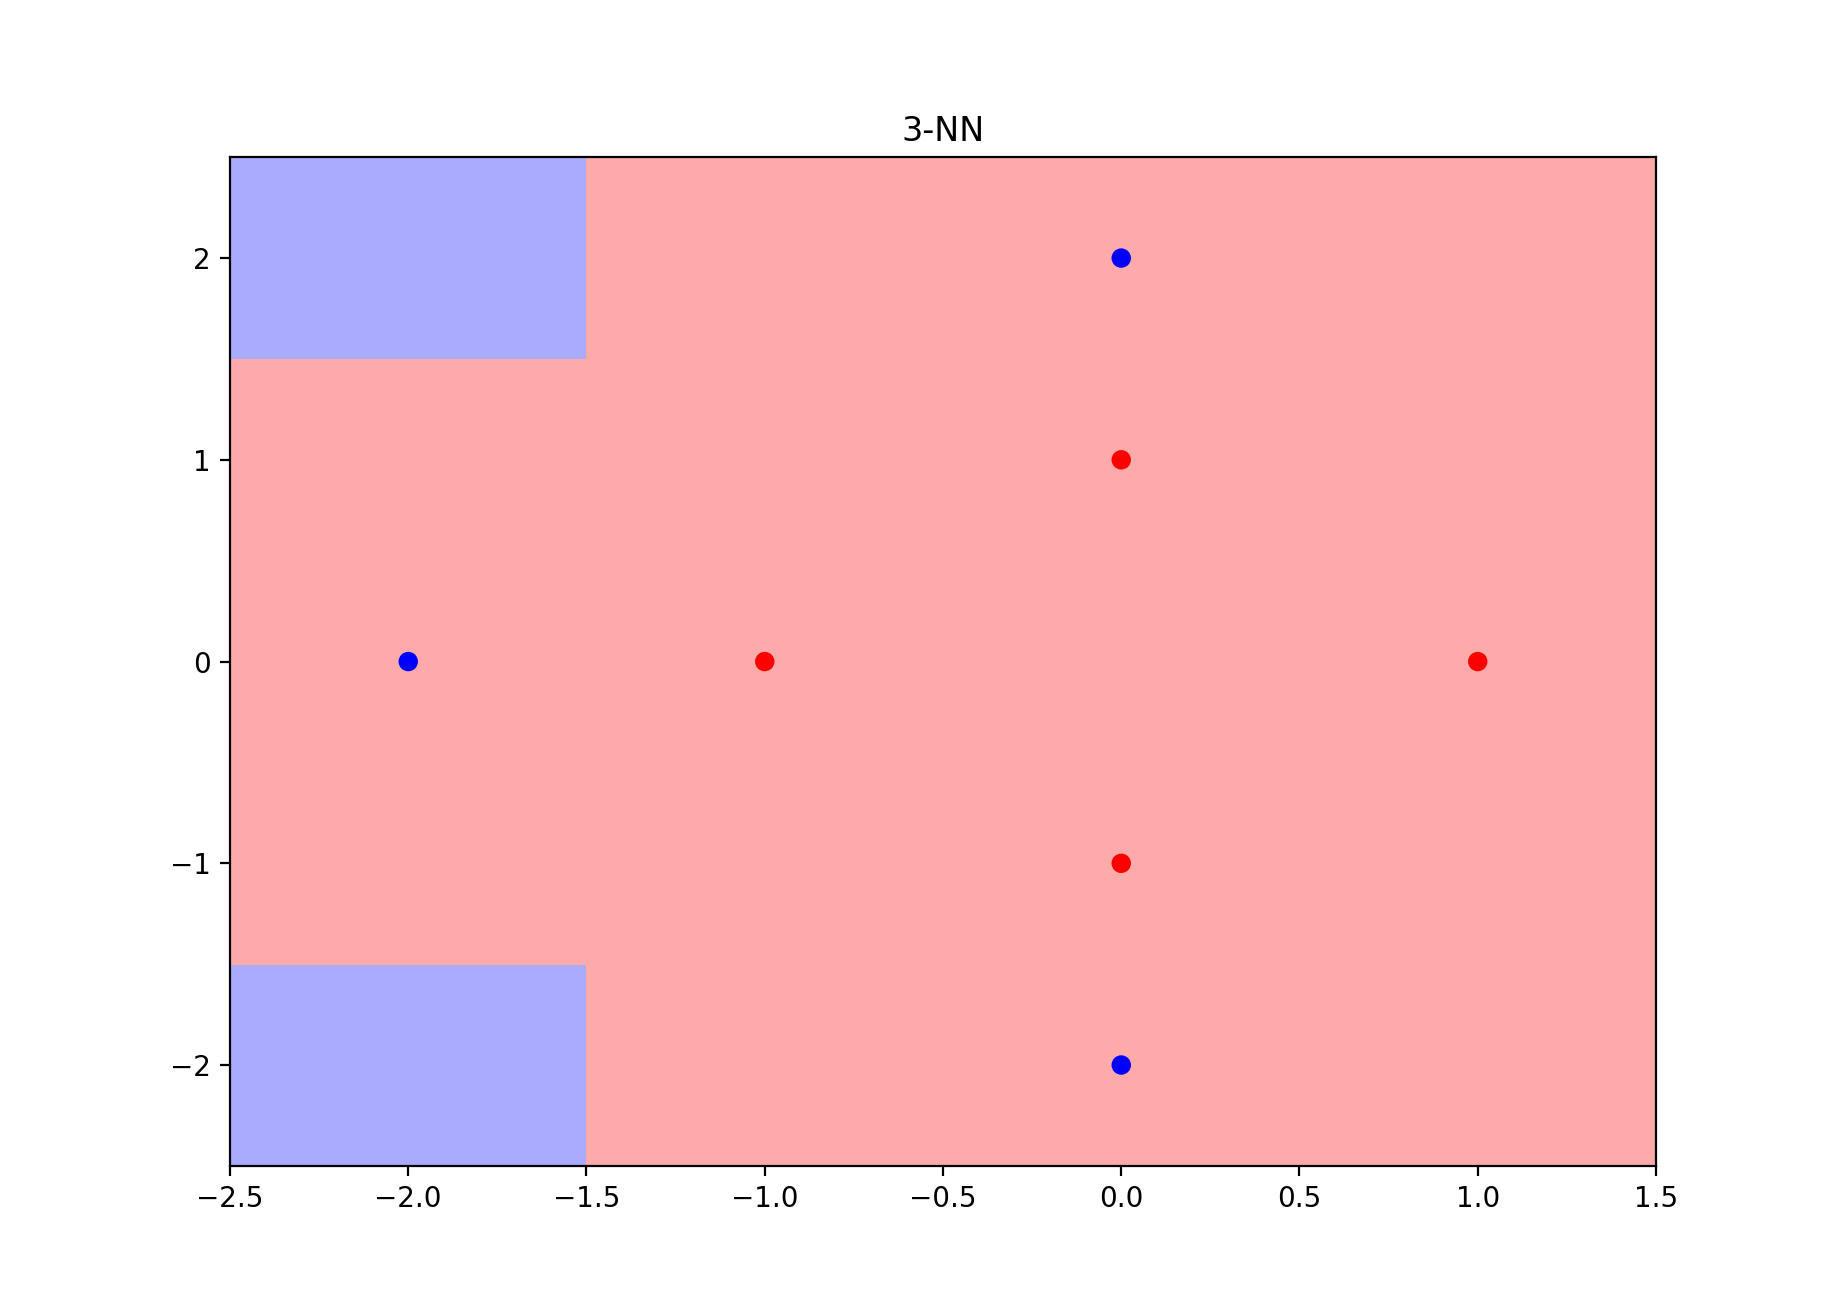
\includegraphics[width=\textwidth]{61a3nn.png}
    \end{center}

  \item \textit{Consider the nonlinear transform $$ \begin{bmatrix} x_1 \\ x_2 \end{bmatrix} 
      \rightarrow \begin{bmatrix} z_1 \\ z_2 \end{bmatrix} = 
        \begin{bmatrix} \sqrt{x_1^2 + x_2^2} \\ \arctan (x_2 / x_1) \end{bmatrix},$$ which 
          maps $\vec{x}$ to $\vec{z}$. Show the classification regions in the $\vec{x}$ space 
          for the 1-NN and 3-NN rules implemented on teh data in the $\vec{z}$-space.}

    First, we have the 1-NN boundary using the transformation.

    \begin{center}
    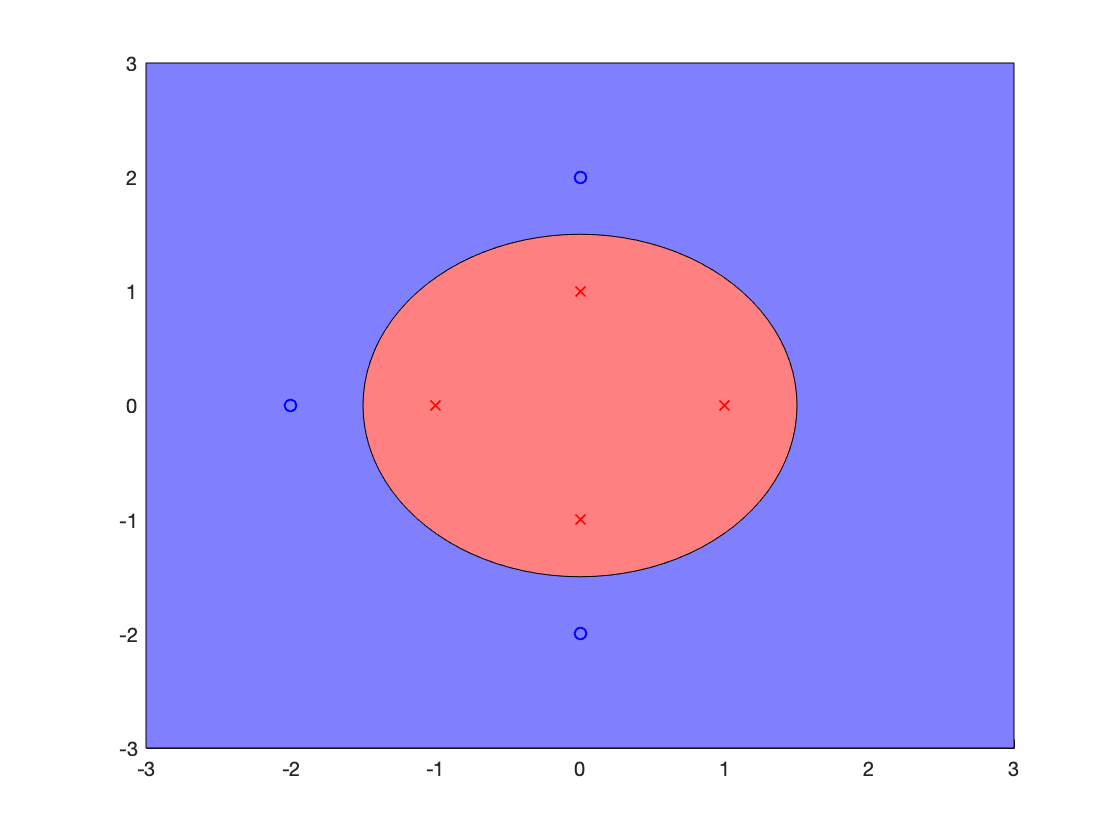
\includegraphics[width=\textwidth]{61b1nn.png}
    \end{center}

    Then, we have the 3-NN boundary under this transformation (excuse the poor plotting; couldn't
    figure out something better in MATLAB).

    \begin{center}
    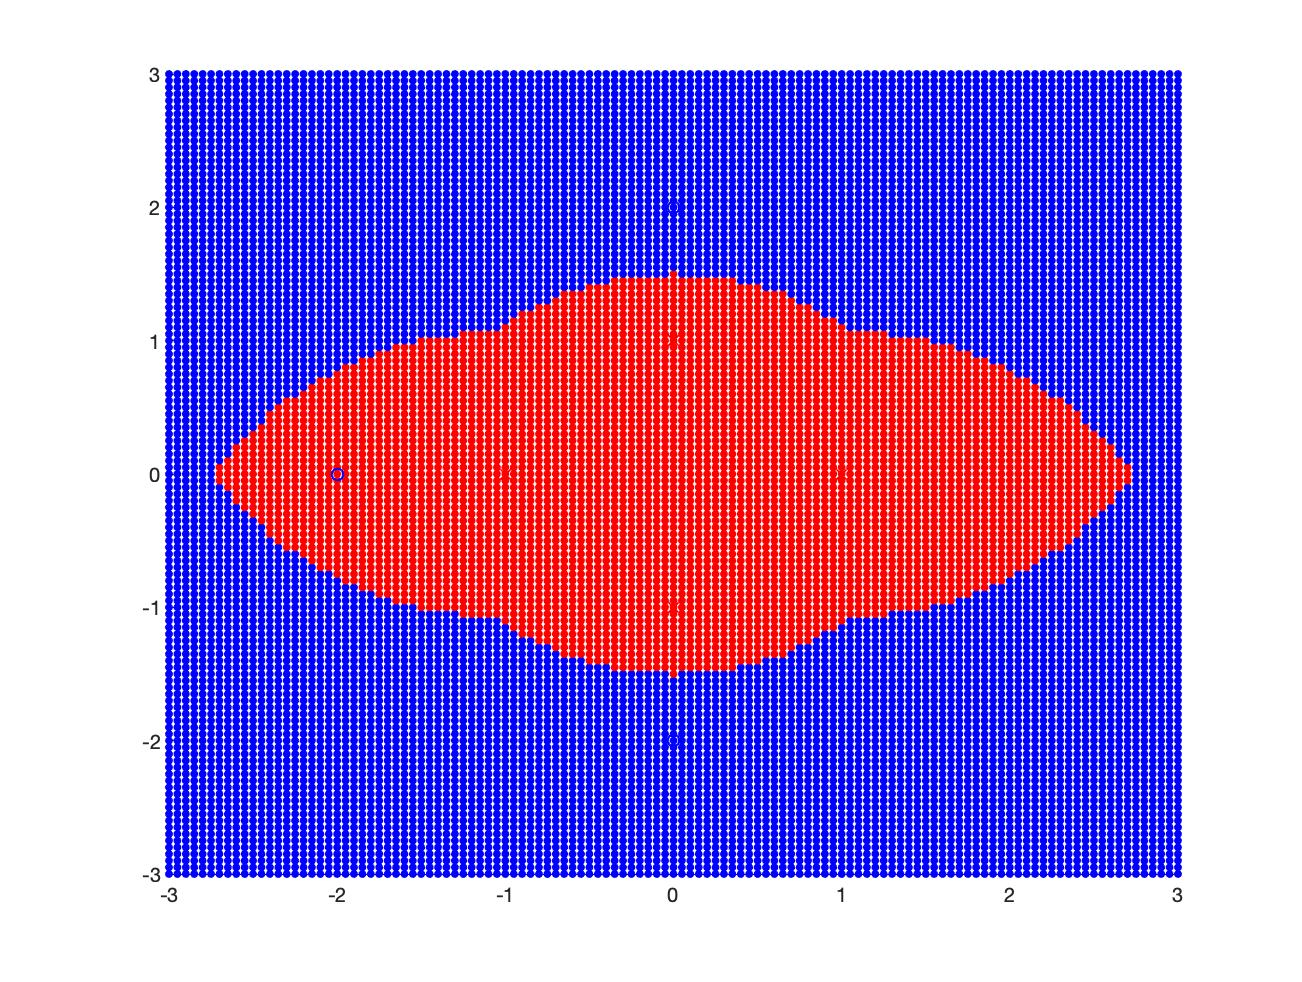
\includegraphics[width=\textwidth]{61b3nn.jpg}
    \end{center}

\end{enumerate}

\subsection*{Problem 6.4}

For the double semi-circle problem in 3.1, plot the decision regions for the 1-NN and 3-NN rules.


\begin{center}
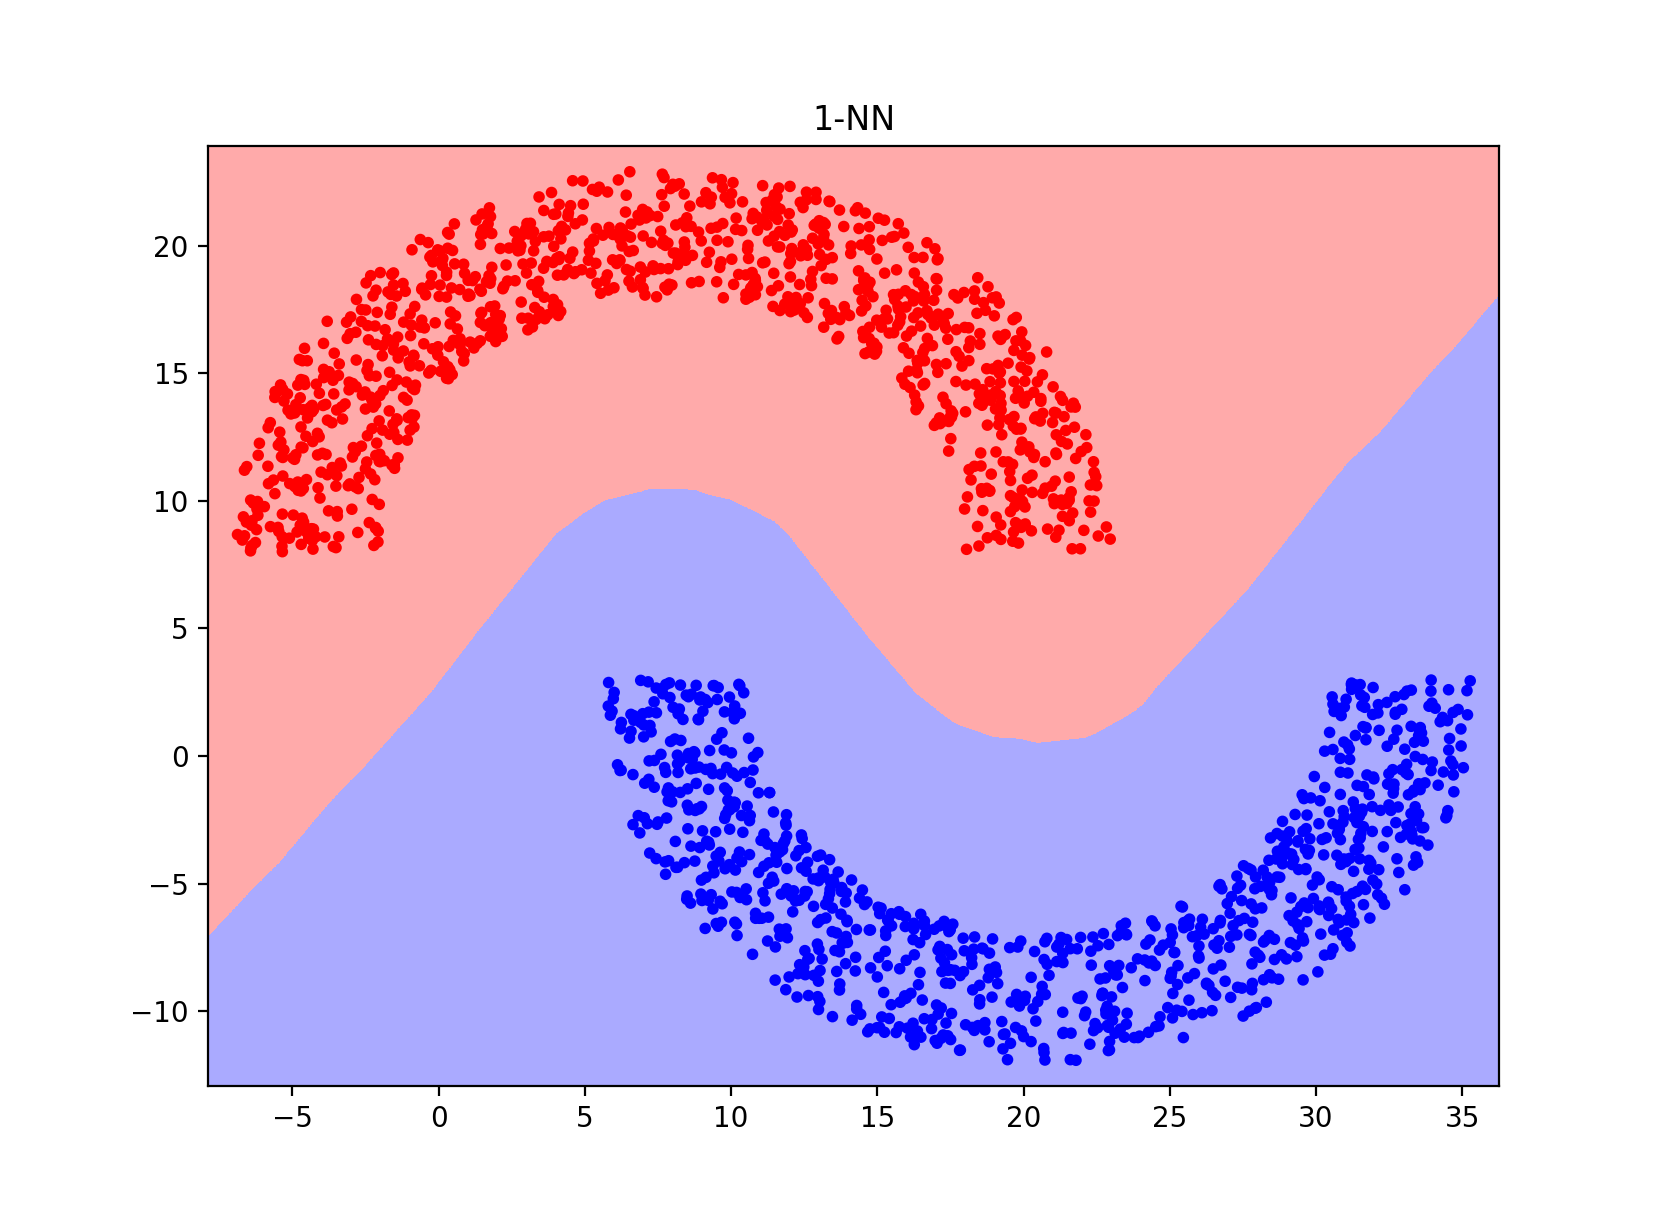
\includegraphics[width=\textwidth]{64-1nn.png}
\end{center}
\begin{center}
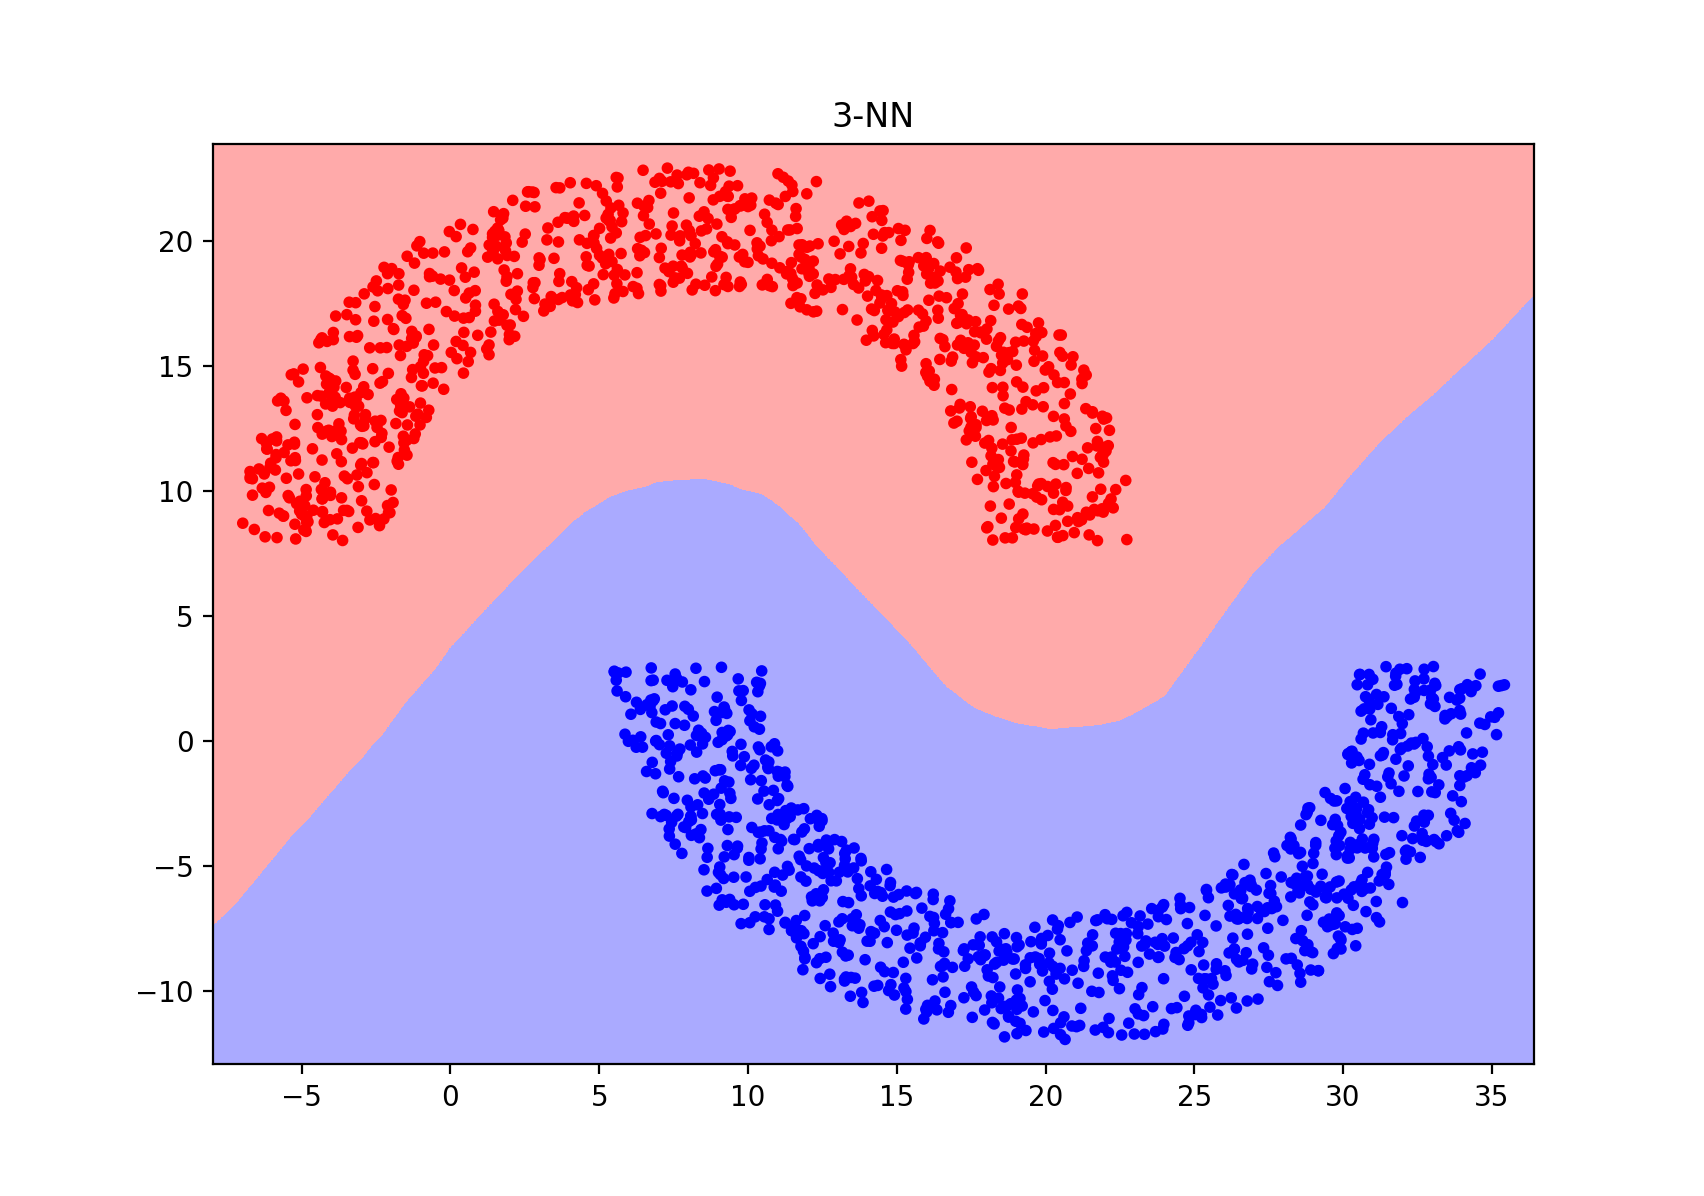
\includegraphics[width=\textwidth]{64-3nn.png}
\end{center}

\subsection*{Problem 6.16}

\begin{enumerate}[(a)]
  \item \textit{Generate a data set of 10,000 data points uniformly in the unit square $[0,1]^2$
    to test the performance of branch and bound method.}

    \begin{enumerate}[i.]
      \item \textit{Construct a 10-partition for the data using the simple greedy heuristic 
        described in the text.}

        \begin{center}
        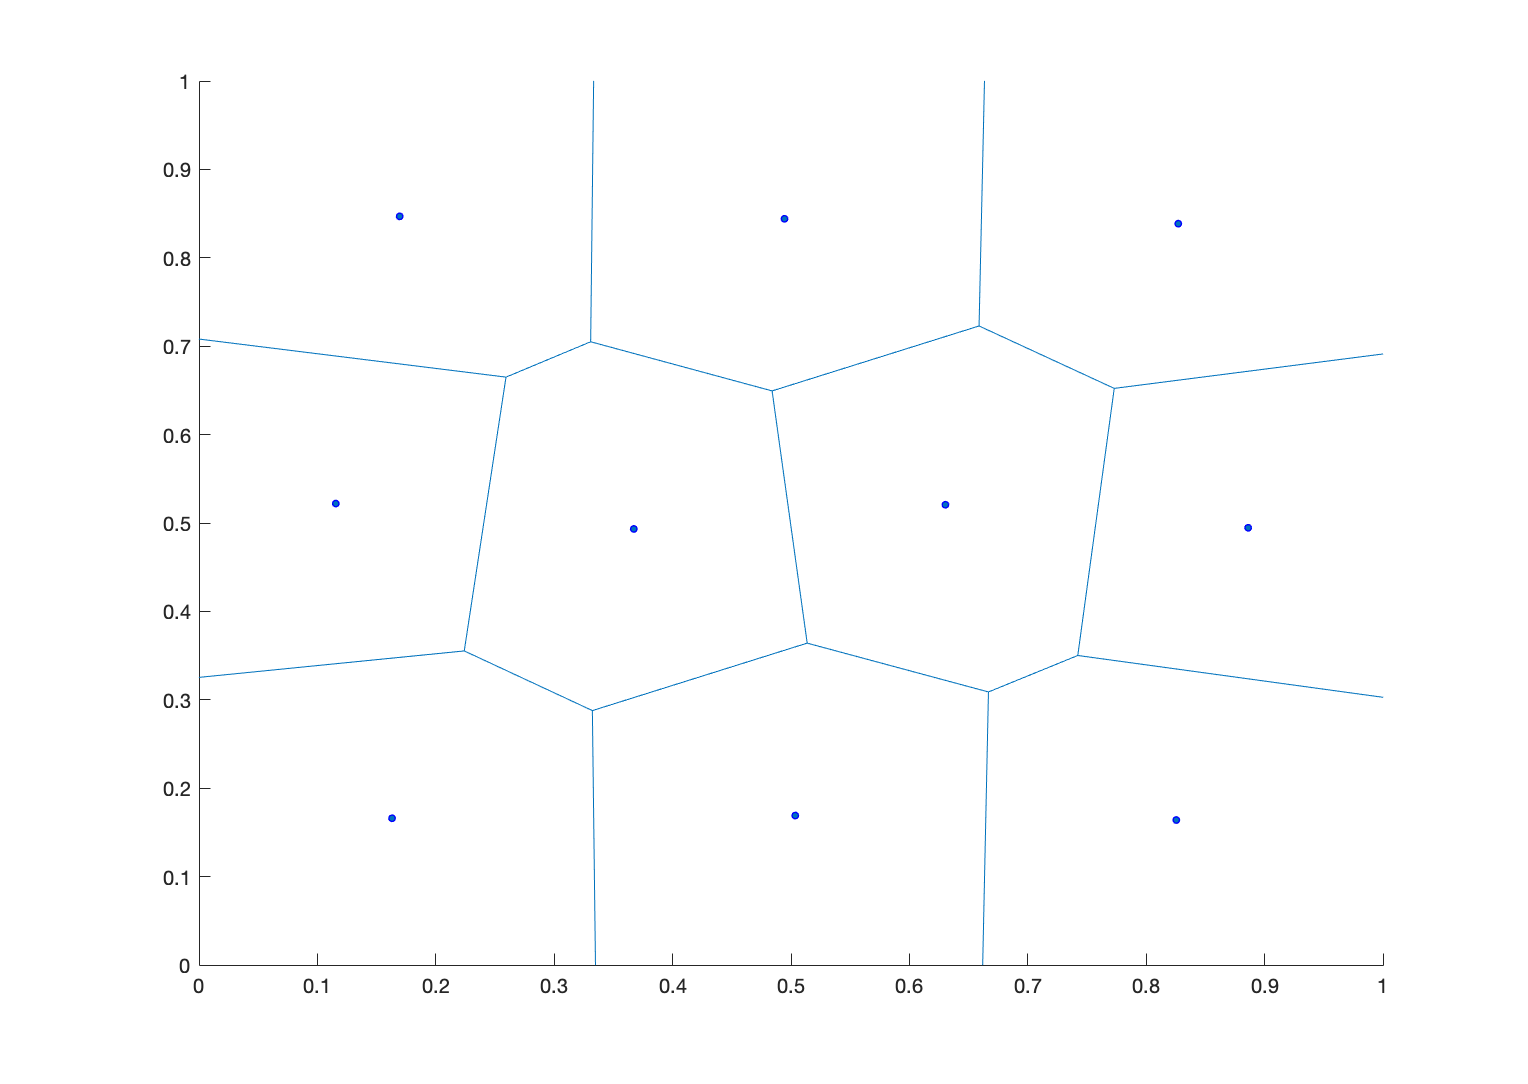
\includegraphics[width=\textwidth]{616ai.png}
        \end{center}

      \item \textit{Generate 10,000 random query points and compare the running time of obtaining
        the nearest neighbor using partition with branch and bound versus brute force approach
        which does not use partition.}

        The brute force approach (finding the minimum of the distances from each query point to
        all other points) takes 3.165 seconds.

        The branch and bound method takes only .397 seconds to find the nearest neighbor for all
        query points.

    \end{enumerate}

  \item \textit{Repeat (a) instead generating the data from a mix of 10 guassians with centers 
    randomly distributed in $[,1]^2$ and identical covariances for each bump equal to $\sigma I$
    where $\sigma = 0.1$.}

    \begin{center}
    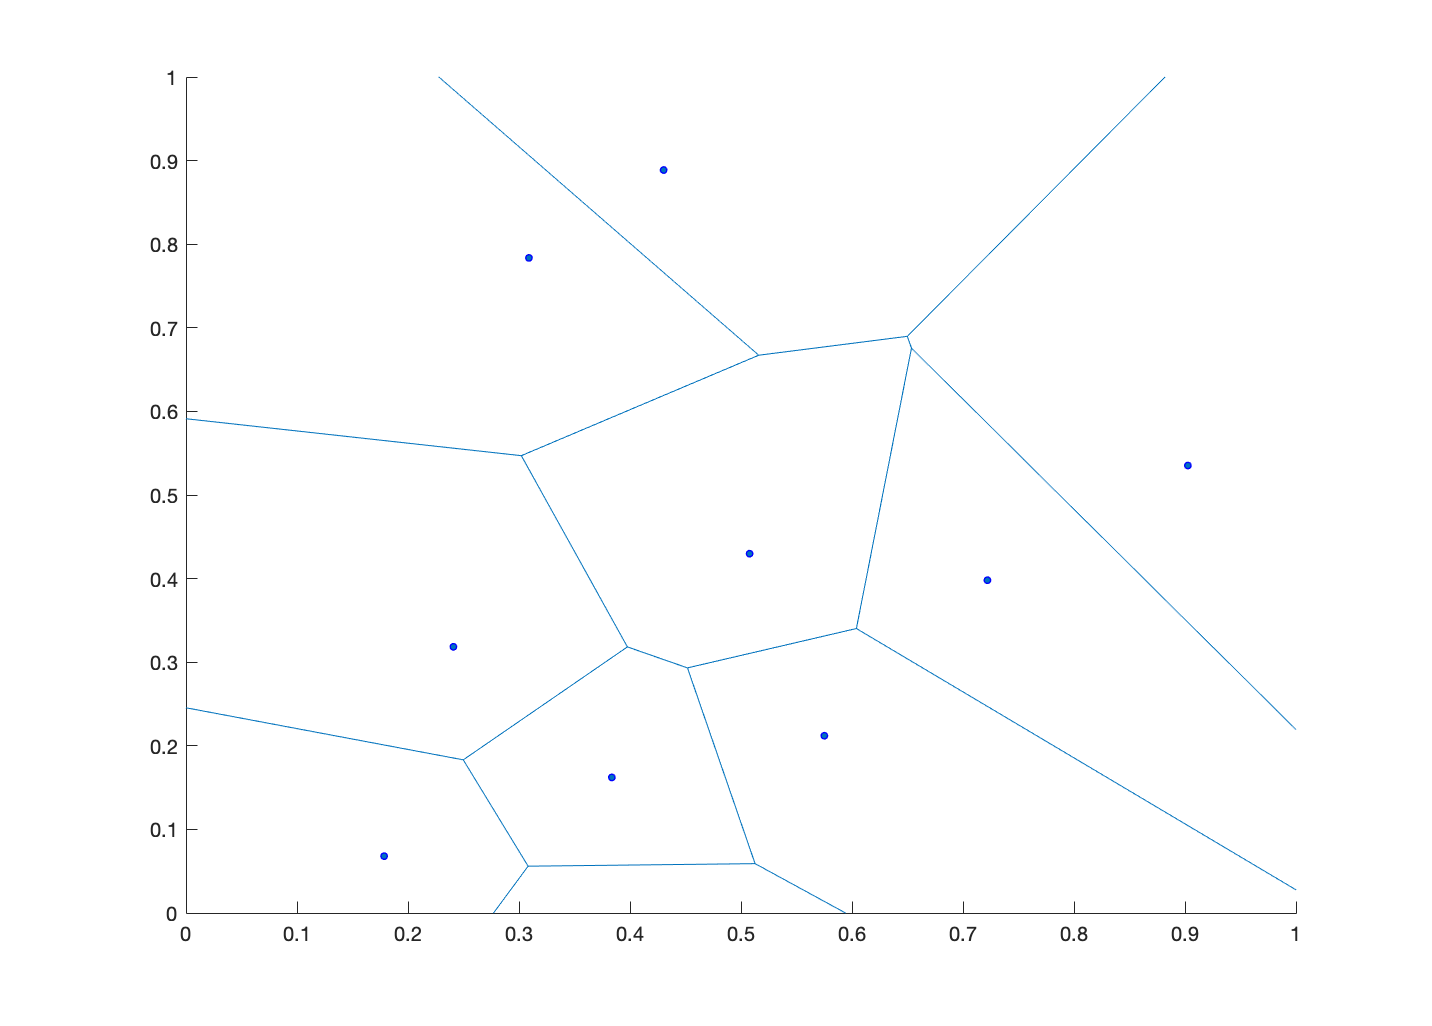
\includegraphics[width=\textwidth]{616bi.png}
    \end{center}

    The brute force method takes about the same amount of time, at 3.214 seconds for all query
    points' nearest neighbors.

    The branch and bound method took slightly less time, at .345 seconds to find all nearest
    neighbors.


  \item \textit{Explain your observations.}

    The guassian distributions lead to much less regular cluster calculations, as you can see from
    the voronoi diagrams. This is because the clusters of points are much more localized, and only
    the centers are randomly distributed, while in part (a) all the points are uniformly 
    distributed, leading to fairly uniform cluster regions.

    The brute force method should take the same amount of time to finish, since it does all the 
    same calculations. It would make sense for the branch and bound method to take less time to
    complete for the guassian distributions, since the bound is more likely to confirm the guess
    for the nearest neighbor when the clusters are tight and more distant. In the uniform 
    distribution, it is much less likely for the bound to hold on the first try, so other clusters
    will have to be analyzed for a nearer neighbor.

  \item \textit{Does your decision to use the branch and bound technique depend on how many test
    points you need to evaluate?}

    Yes. For only a few test points, the brute force method may be the faster approach because it
    takes a fairly significant amount of computation to calculate all the clusters and perform the
    bound test. However, as the number of test points increases, the branch and bound method will
    outpace brute force.

\end{enumerate}






\end{document}
